\chapter{Results}
After having spoken of the many maintenance and code quality advantages of version 5, this chapter includes some benchmarks made on the library, in particular it compares version 4 with version 5. All measurements were performed on a custom built PC running Linux, all virtualised in a Docker environment, specifically with the following Dockerfile:
\begin{minted}{Dockerfile}
# Use the official Swift image from Docker Hub
FROM swift:5.10-jammy

# Set the working directory inside the container
WORKDIR /app

# Copy the current directory contents into the container at /app
COPY . .

# Download Swift package dependencies
RUN swift package resolve

# Command to run the application
CMD ["swift", "package", "--allow-writing-to-package-directory", "benchmark", "--format", "jmh"]
\end{minted}
For benchmarking, the package-benchmark library was used \cite{package-benchmark}. The benchmarks test signing, verification and token lifecycle, which includes key creation, signing and verification, using different algorithms and calculating different parameters:
\begin{itemize}
    \item throughput: number of operations per second;
    \item \latexinline{malloc}s: number of memory allocations, indicates effective memory usage.
\end{itemize}
HMAC was left out because version 5 uses the same implementation as version 4, therefore the comparison is not really useful. PSS was also not considered as it was not present in version 4. Additionally, total lines of code were also measured.
Obviously the code is built using release mode, which optimises performance at the expense of build time and binary size.


\section{Signing}
This section shows the signing benchmarks is done. For each test, a key is constructed once, and then used to sign a token multiple times.

\subsection*{Version 4}
Version 4 was tested using this code:
\begin{minted}{swift}
Benchmark("ES256") { benchmark in
    for _ in benchmark.scaledIterations {
        let signer = try JWTSigner.es256(key: .generate())
        let token = try await signer.sign(payload)
        _ = try await signer.verify(token, as: Payload.self)
    }
}
\end{minted}

\subsection*{Version 5}
This is the code that was executed using version 5, is equivalent to version 4 from above:
\begin{minted}{swift}
Benchmark("ES256") { benchmark in
    let key = ES256PrivateKey()
    let keyCollection = await JWTKeyCollection().addES256(key: key)
    for _ in benchmark.scaledIterations {
        _ = try await keyCollection.sign(payload)
    }
}
\end{minted}

\subsection*{Results}
Following are the results.
\subsubsection*{Performance}
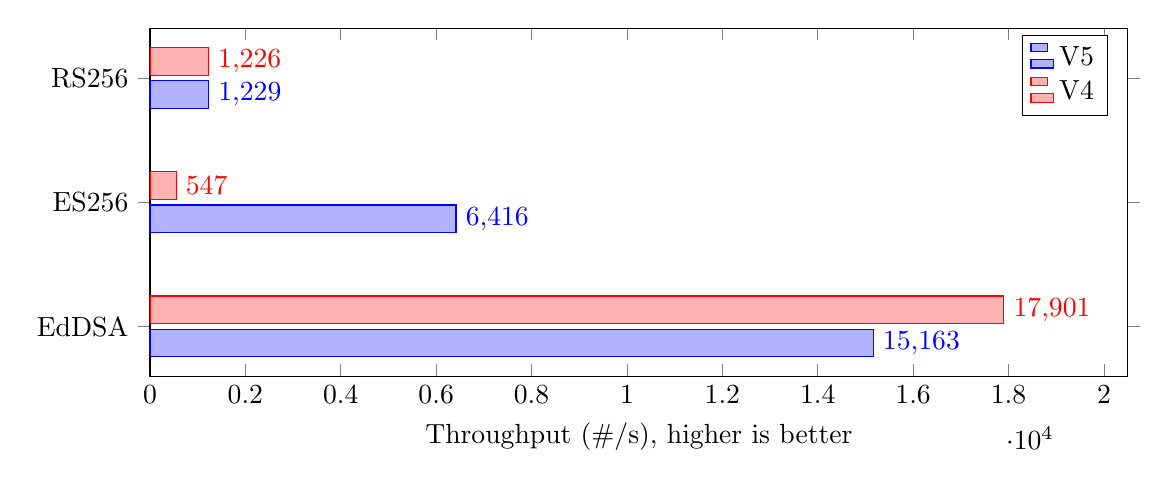
\begin{tikzpicture}
\begin{axis}[
    xbar, % This option is used for horizontal bars
    xmin=0, % Minimum value on the x-axis
    xmax=20500,
    width=14cm, height=6cm, % Width and height of the bar chart
    enlarge y limits=0.2, % Adds some padding between the bars
    xlabel={Throughput (\#/s), higher is better}, % Label for the x-axis
    symbolic y coords={
        EdDSA,
        ES256,
        RS256
    }, % Define the items/categories
    ytick=data, % Ensure there's a tick for each symbolic y coord
    nodes near coords, % Show the value near each bar
    nodes near coords align={horizontal}, % Align the value label properly for horizontal bars
]
\addplot 
	coordinates {
        (1229,RS256)
        (15163,EdDSA) 
        (6416,ES256)
    };
\addplot 
	coordinates {
        (1226,RS256)
        (17901,EdDSA) 
        (547,ES256)
    };
\legend{V5, V4}
\end{axis}
\end{tikzpicture} \\
This chart shows the total number of operations performed per second.
From the chart, the first noticeable thing is how slow both versions of the RS256 algorithm are compared to the elliptic curves ones. A significant improvement was made in signing using the ES256 algorithm and finally a noticeable regression in signing through EdDSA.
\begin{table}[h]
    \centering
    \begin{tabular}{lccr}
        \toprule
        Algorithm & Version 4 & Version 5 & \multicolumn{1}{c}{Change} \\
        \midrule
        RS256 & 1229 & 1226 & \textcolor{darkergreen}{+0.24\%} \\
        ES256 & 6416 & 547 & \textcolor{darkergreen}{+1072.94\%} \\
        EdDSA & 15163 & 17901 & \textcolor{darkerred}{-15.3\%} \\
        \bottomrule
    \end{tabular}
    \caption{Signing throughput (\#/s) difference}
\end{table}

\subsubsection*{Memory Management}

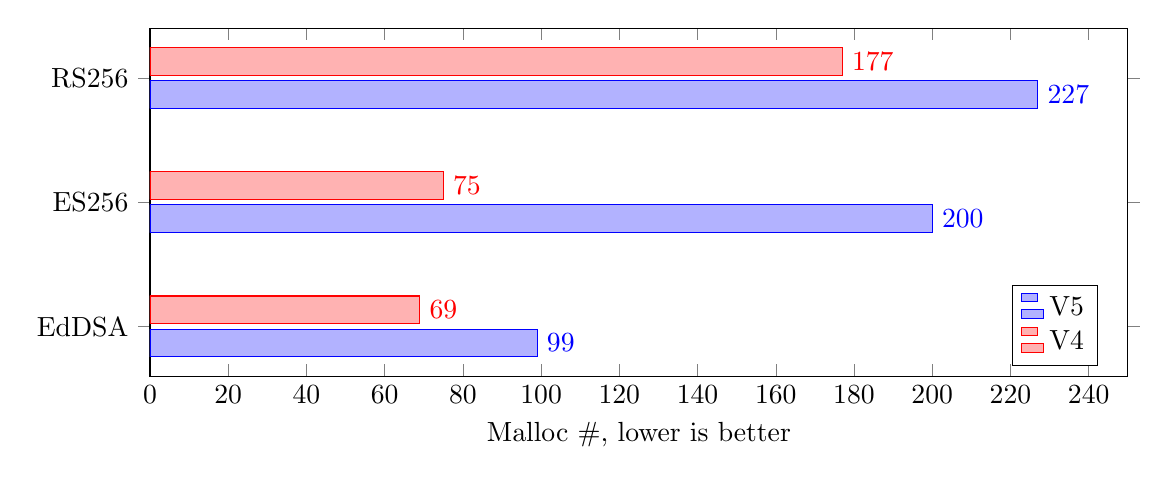
\begin{tikzpicture}
\begin{axis}[
    xbar, % This option is used for horizontal bars
    xmin=0, % Minimum value on the x-axis
    xmax=250,
    width=14cm, height=6cm, % Width and height of the bar chart
    enlarge y limits=0.2, % Adds some padding between the bars
    xlabel={Malloc \#, lower is better}, % Label for the x-axis
    legend pos=south east, % Position the legend at the bottom right
    symbolic y coords={
        EdDSA,
        ES256,
        RS256
    }, % Define the items/categories
    ytick=data, % Ensure there's a tick for each symbolic y coord
    nodes near coords, % Show the value near each bar
    nodes near coords align={horizontal}, % Align the value label properly for horizontal bars
]
\addplot 
	coordinates {
        (227,RS256)
        (99,EdDSA) 
        (200,ES256)
    };
\addplot 
	coordinates {
        (177,RS256)
        (69,EdDSA) 
        (75,ES256)
    };
\legend{V5, V4}
\end{axis}
\end{tikzpicture} \\
This graph shows the total number of memory allocations.
Just as before, RSA is outperformed by the elliptic curve algorithms, though not by much if inspecting the ES256 algorithm. EdDSA is the clear winner, though all three algorithms saw a regression in version 5. This is likely due to the usage of Swift types to get to C rather than directly accessing C constructs.
\begin{table}[h]
    \centering
    \begin{tabular}{lccr}
        \toprule
        Algorithm & Version 4 & Version 5 & \multicolumn{1}{c}{Change} \\
        \midrule
        RS256 & 177 & 227 & \textcolor{darkerred}{+26.28\%} \\
        ES256 & 75 & 200 & \textcolor{darkerred}{+166.67\%} \\
        EdDSA & 69 & 99 & \textcolor{darkerred}{+47.76\%} \\
        \bottomrule
    \end{tabular}
    \caption{Signing \latexinline{malloc} (\#) difference }
\end{table}

\section{Verification}
Version 5 saw a big drop in signature verification efficiency.

\subsection*{Version 4}
This is the code used to verify a token using JWTKit 4:
\begin{minted}{swift}
Benchmark("ES256") { benchmark in
    let pem = """
    -----BEGIN PUBLIC KEY-----
    MFkwEwYHKoZIzj0CAQYIKoZIzj0DAQcDQgAEEVs/o5+uQbTjL3chynL4wXgUg2R9
    q9UU8I5mEovUf86QZ7kOBIjJwqnzD1omageEHWwHdBO6B+dFabmdT9POxg==
    -----END PUBLIC KEY-----
    """
    let token = "eyJhbGciOiJFUzI1NiIsInR5cCI6IkpXVCJ9.
        eyJuYW1lIjoiSm9obiBEb2UiLCJhZG1pbiI6dHJ1ZX0.
        vY4BbTLWcVbA4sS_EnaSV-exTZT3mRpH6JNc5C7XiUDA1PfbTO6LdO
        bMFYPEcKZMydfHy6SJz1eJySq2uYBLAA"
    let signer = try JWTSigner.es256(key: .public(pem: pem))
    for _ in benchmark.scaledIterations {
        _ = try signer.verify(token, as: Payload.self)
    }
}
\end{minted}

\subsection*{Version 5}
This on the other hand is what was used in version 5:
\begin{minted}{swift}
Benchmark("ES256") { benchmark in
    let pem = """
    -----BEGIN PUBLIC KEY-----
    MFkwEwYHKoZIzj0CAQYIKoZIzj0DAQcDQgAEEVs/o5+uQbTjL3chynL4wXgUg2R9
    q9UU8I5mEovUf86QZ7kOBIjJwqnzD1omageEHWwHdBO6B+dFabmdT9POxg==
    -----END PUBLIC KEY-----
    """
    let token = "eyJhbGciOiJFUzI1NiIsInR5cCI6IkpXVCJ9.
    eyJuYW1lIjoiSm9obiBEb2UiLCJhZG1pbiI6dHJ1ZX0.
    vY4BbTLWcVbA4sS_EnaSV-exTZT3mRpH6JNc5C7XiUDA1PfbTO
    6LdObMFYPEcKZMydfHy6SJz1eJySq2uYBLAA"
    let key = try ES256PublicKey(pem: pem)
    let keyCollection = await JWTKeyCollection().addES256(key: key)
    for _ in benchmark.scaledIterations {
        _ = try await keyCollection.verify(token, as: Payload.self)
    }
}
\end{minted}

\subsection*{Results}
\subsubsection*{Performance}
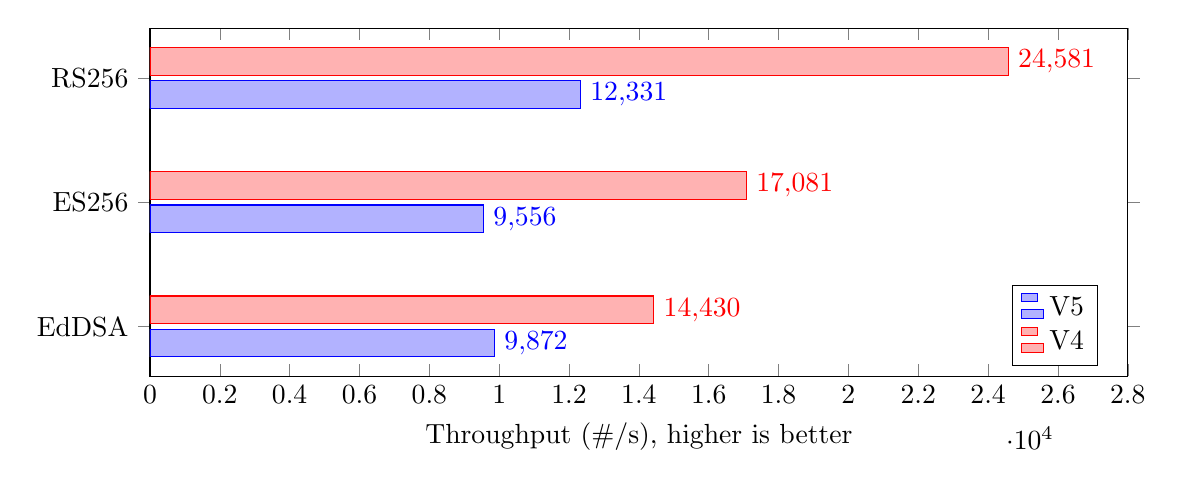
\begin{tikzpicture}
\begin{axis}[
    xbar, % This option is used for horizontal bars
    xmin=0, % Minimum value on the x-axis
    xmax=28000,
    width=14cm, height=6cm, % Width and height of the bar chart
    enlarge y limits=0.2, % Adds some padding between the bars
    xlabel={Throughput (\#/s), higher is better}, % Label for the x-axis
    legend pos=south east, % Position the legend at the bottom right
    symbolic y coords={
        EdDSA,
        ES256,
        RS256
    }, % Define the items/categories
    ytick=data, % Ensure there's a tick for each symbolic y coord
    nodes near coords, % Show the value near each bar
    nodes near coords align={horizontal}, % Align the value label properly for horizontal bars
]
\addplot 
	coordinates {
        (12331,RS256)
        (9872,EdDSA) 
        (9556,ES256)
    };
\addplot 
	coordinates {
        (24581,RS256)
        (14430,EdDSA) 
        (17081,ES256)
    };
\legend{V5, V4}
\end{axis}
\end{tikzpicture} \\
The chart shows a significant drop in throughput when using version 5. The RS256 algorithm sees its throughput halved in version 5. While the EC algorithms are not as drastic, the decrease is still noticeable and is likely due to the addition of code layers. 

\begin{table}[h]
    \centering
    \begin{tabular}{lccr}
        \toprule
        Algorithm & Version 4 & Version 5 & \multicolumn{1}{c}{Change} \\
        \midrule
        RS256 & 24,581 & 12,331 & \textcolor{darkerred}{-99.34\%} \\
        ES256 & 17,081 & 9,556 & \textcolor{darkerred}{-78.75\%} \\
        EdDSA & 14,430 & 9,872 & \textcolor{darkerred}{-46.17\%} \\
        \bottomrule
    \end{tabular}
    \caption{Verification \latexinline{throughput} (\#/s) difference}
\end{table}

\subsubsection*{Memory Management}

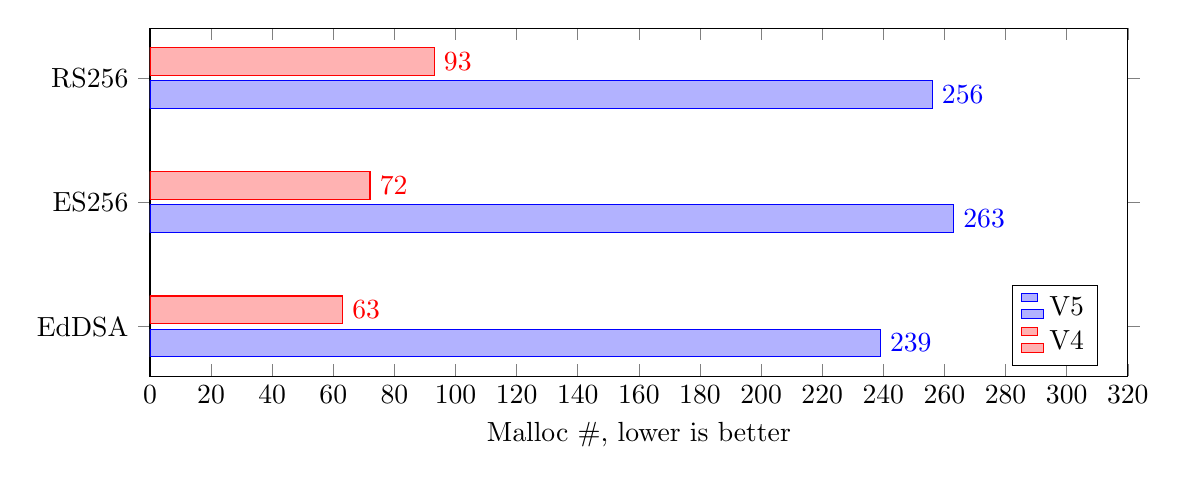
\begin{tikzpicture}
\begin{axis}[
    xbar, % This option is used for horizontal bars
    xmin=0, % Minimum value on the x-axis
    xmax=320,
    width=14cm, height=6cm, % Width and height of the bar chart
    enlarge y limits=0.2, % Adds some padding between the bars
    xlabel={Malloc \#, lower is better}, % Label for the x-axis
    legend pos=south east, % Position the legend at the bottom right
    symbolic y coords={
        EdDSA,
        ES256,
        RS256
    }, % Define the items/categories
    ytick=data, % Ensure there's a tick for each symbolic y coord
    nodes near coords, % Show the value near each bar
    nodes near coords align={horizontal}, % Align the value label properly for horizontal bars
]
\addplot 
	coordinates {
        (256,RS256)
        (239,EdDSA) 
        (263,ES256)
    };
\addplot 
	coordinates {
        (93,RS256)
        (63,EdDSA) 
        (72,ES256)
    };
\legend{V5, V4}
\end{axis}
\end{tikzpicture} \\
The chart above shows memory allocations. It shows a clear increase in memory usage from all three algorithms, and as before it is likely due to the fact that the new version uses safer and more abstract that increase memory footprint but also improve maintainability and security.

\begin{table}[h]
    \centering
    \begin{tabular}{lccr}
        \toprule
        Algorithm & Version 4 & Version 5 & \multicolumn{1}{c}{Change} \\
        \midrule
        RS256 & 93 & 256 & \textcolor{darkerred}{+175.27\%} \\
        ES256 & 72 & 263 & \textcolor{darkerred}{+265.28\%} \\
        EdDSA & 63 & 238 & \textcolor{darkerred}{+279.365\%} \\
        \bottomrule
    \end{tabular}
    \caption{Verification \latexinline{malloc} (\#) difference }
\end{table} 

\section{Token Lifecycle}
Finally, this section sheds light on a more real life usage of the tokens, which includes both token signing and verification and also key creation. Since keys can be created different ways, it's correct for these ways to be differently measured, therefore the following graphs will be slightly more complex. Following are code examples which showcase how data was gathered.

\subsection*{Version 4}
\begin{minted}{swift}
Benchmark("ES256 Generated") { benchmark in
    for _ in benchmark.scaledIterations {
        let signer = try JWTSigner.es256(key: .generate())
        let token = try await signer.sign(payload)
        _ = try await signer.verify(token, as: Payload.self)
    }
}
\end{minted}

\subsection*{Version 5}
\begin{minted}{swift}
Benchmark("ES256 Generated") { benchmark in
    for _ in benchmark.scaledIterations {
        let key = ES256PrivateKey()
        let keyCollection = await JWTKeyCollection().addES256(key: key)
        let token = try await keyCollection.sign(payload)
        _ = try await keyCollection.verify(token, as: Payload.self)
    }
}
\end{minted}

\subsection*{Results}

\subsubsection*{Performance}
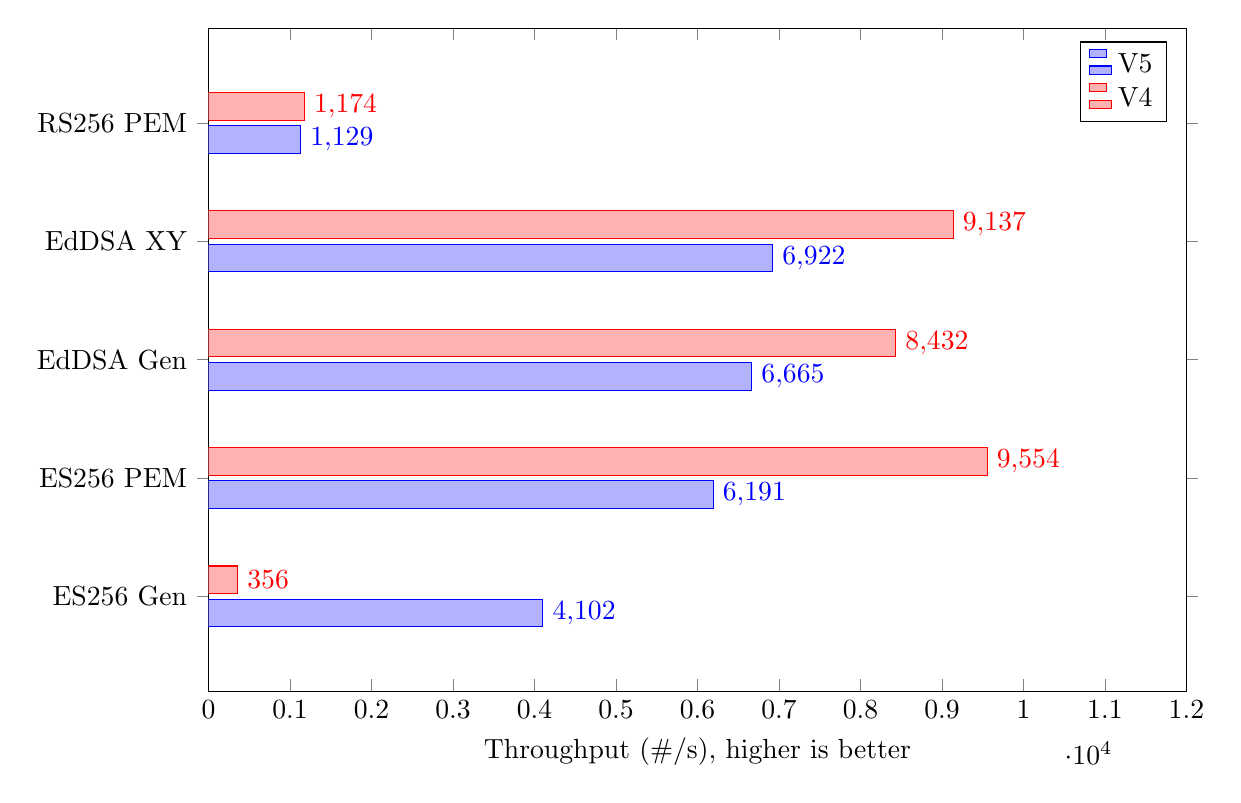
\begin{tikzpicture}
\begin{axis}[
    xbar, % This option is used for horizontal bars
    xmin=0, % Minimum value on the x-axis
    xmax=12000,
    width=14cm, height=10cm, % Width and height of the bar chart
    enlarge y limits=0.2, % Adds some padding between the bars
    xlabel={Throughput (\#/s), higher is better}, % Label for the x-axis
    symbolic y coords={
        ES256 Gen,
        ES256 PEM,
        EdDSA Gen,
        EdDSA XY,
        RS256 PEM
    }, % Define the items/categories
    ytick=data, % Ensure there's a tick for each symbolic y coord
    nodes near coords, % Show the value near each bar
    nodes near coords align={horizontal}, % Align the value label properly for horizontal bars
]
\addplot
    coordinates {
        (1129,RS256 PEM)
        (6665,EdDSA Gen) 
        (4102,ES256 Gen) 
        (6922,EdDSA XY) 
        (6191,ES256 PEM)
    };
\addplot 
	coordinates {
        (1174,RS256 PEM)
        (8432,EdDSA Gen) 
        (356,ES256 Gen) 
        (9137,EdDSA XY) 
        (9554,ES256 PEM)
    };
\legend{V5, V4}
\end{axis}
\end{tikzpicture} \\
There is a substantial decrease in performance in the elliptic curves algorithms, except in the generated version of ES256, which doesn't use a \gls{pem} file but instead creates a key on the fly. RS256 performance on the other hand remains constant and, as usual, behind the rest.

\begin{table}[h]
    \centering
    \begin{tabular}{lccr}
        \toprule
        Algorithm & Version 4 & Version 5 & \multicolumn{1}{c}{Change} \\
        \midrule
        RS256 & 1,174 & 1,129 & \textcolor{darkerred}{-3,83\%} \\
        EdDSA XY & 9,137 & 6,922 & \textcolor{darkerred}{-24.24\%} \\
        EdDSA Gen & 8,432 & 6,665 & \textcolor{darkerred}{-20.96\%} \\
        ES256 PEM & 9,554 & 6,191 & \textcolor{darkerred}{-35.2\%} \\
        ES256 Gen & 356 & 4,102 & \textcolor{darkergreen}{+1052.25\%} \\
        \bottomrule
    \end{tabular}
    \caption{Token lifecycle throughput (\#/s) difference}
\end{table} 

\subsubsection*{Memory Management}
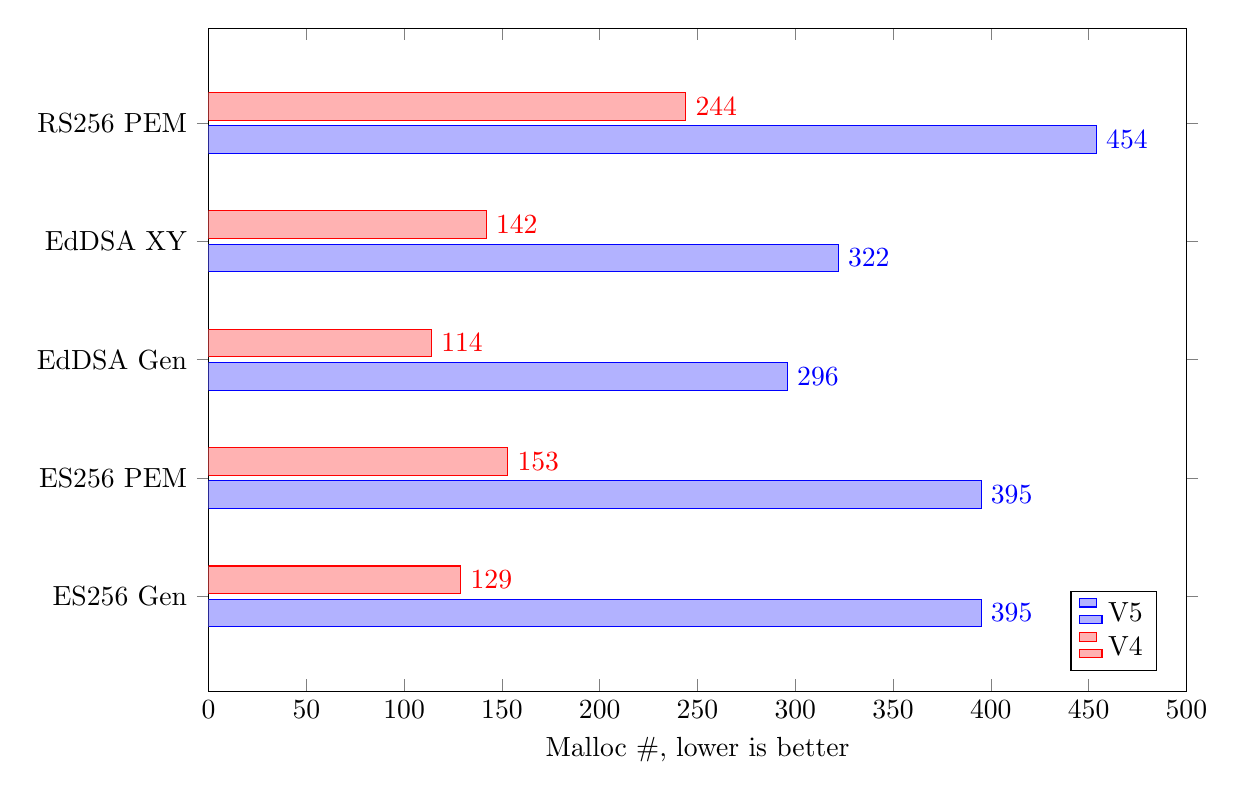
\begin{tikzpicture}
\begin{axis}[
    xbar, % This option is used for horizontal bars
    xmin=0, % Minimum value on the x-axis
    xmax=500,
    width=14cm, height=10cm, % Width and height of the bar chart
    enlarge y limits=0.2, % Adds some padding between the bars
    xlabel={Malloc \#, lower is better}, % Label for the x-axis
    legend pos=south east, % Position the legend at the bottom right
    symbolic y coords={
        ES256 Gen,
        ES256 PEM,
        EdDSA Gen,
        EdDSA XY,
        RS256 PEM
    }, % Define the items/categories
    ytick=data, % Ensure there's a tick for each symbolic y coord
    nodes near coords, % Show the value near each bar
    nodes near coords align={horizontal}, % Align the value label properly for horizontal bars
]
\addplot
    coordinates {
        (454,RS256 PEM)
        (296,EdDSA Gen) 
        (395,ES256 Gen) 
        (322,EdDSA XY) 
        (395,ES256 PEM)
    };
\addplot 
	coordinates {
        (244,RS256 PEM)
        (114,EdDSA Gen) 
        (129,ES256 Gen) 
        (142,EdDSA XY) 
        (153,ES256 PEM)
    };
\legend{V5, V4}
\end{axis}
\end{tikzpicture} \\
Finally, this chart shows the total memory allocations which happened during the tests. This also shows a demerit for version 5, as there's much more memory usage with SwiftCrypto. This is likely due to the added complexity and abstraction of the code.
\begin{table}[ht]
    \centering
    \begin{tabular}{lccr}
        \toprule
        Algorithm & Version 4 & Version 5 & \multicolumn{1}{c}{Change} \\
        \midrule
        RS256 & 244 & 454 & \textcolor{darkerred}{+86.07\%} \\
        EdDSA XY & 142 & 322 & \textcolor{darkerred}{+126.76\%} \\
        EdDSA Gen & 114 & 296 & \textcolor{darkerred}{+159.65\%} \\
        ES256 PEM & 153 & 395 & \textcolor{darkerred}{+158.17\%} \\
        ES256 Gen & 129 & 395 & \textcolor{darkergreen}{+206.20\%} \\
        \bottomrule
    \end{tabular}
    \caption{Token lifecycle \latexinline{malloc} (\#) difference}
\end{table}

\section{Lines of Code}
While benchmarks indicate a big gap in performance between the two versions, this will likely change with the passing of time and the gradual updating of the package, the beginning of which can be seen in Swift 5.10, which brings new features (such as \swiftinline{~Copyable}) that can enhance performance. One  change that can be seen immediately on the other hand is the size of the package, which decreased considerably in version 5. In particular, using the cloc package \cite{cloc}, the results were the following:
\begin{table}[ht]
    \centering
    \begin{tabular}{ccr}
        \toprule
        Version 4 & Version 5 & Change \\
        \midrule
        311897 & 3160 & \textcolor{darkergreen}{-98.99\%} \\
        \bottomrule
    \end{tabular}
    \caption{Lines of code (\#) difference }
\end{table} \\
This table indicates the total number of code lines in the project, before and after the transition to version 5. The difference is massive as the whole vendored version of BoringSSL is gone. 

\section{End result}
While the benchmark results do not look good for version 5 of JWTKit, this is an acceptable result as code quality is greatly increased and with the latest Swift versions concurrency is ensured. A good example of code quality improvement is the drastic decrease in lines of code, and therefore quantity of code that has to be maintained. This also allows easier development and thus performance can be improved more easily, without having to touch low level C code. 
